Um Webservices dynamisch verwenden zu können, muss eine Architektur in der Lage sein, diese erst zur Laufzeit zu binden. In diesem Abschnitt wird gezeigt, wie eine Architektur aufgebaut sein muss, in der die dynamische Bindung von semantischen Webservice möglich ist.

\bigskip

Wie Dostal und Jeckle in \cite[S.61]{xmlspek4} ausführen, werden in den üblichen Beschreibungen zum Ablauf in einem Web-Service-Szenario \ac{WSDL}-Dokumente hauptsächlich als Eingabe für einen Generator verwendet, mit dessen Hilfe die programmierspezifischen Implementierungen erzeugt werden. Dies erfolgt allerdings in der Regel zur Entwicklungszeit der Anwendung und nicht zu deren Laufzeit. Zwar ist es bei Sprach- und Ausführungsumgebungen wie Java heute technisch durchaus möglich, auch zur Ausführungszeit Klassen der Anwendung hinzuzufügen und auf diesem Weg das oben beschriebene Implementierungszenario von der Entwicklungs- in die Laufzeit zu verlagern. Allerdings würde ein solcher Ansatz eine Reihe von Nachteilen bzw. Riksiken bergen. Das gewichtigste Argument gegen den Genierungsansatz ist zweifelsfrei im Bereich Sicherheit angesiedelt. Das Einbinden von nicht getestetem Code bietet Angreifern ein \emph{el Dorada} von Möglichkeiten, potentiell gefährliche Programmsequenzen in die Anwendung ein zu schmuggeln. Statt des generativen Ansatzes eignet sich daher ein Framework besser, das mit Hilfe der Informationen in einem \ac{WSDL}-Dokument eine \ac{SOAP}-Kommunikation durchführen kann, ohne dazu Codegenerierungen durchführen zu müssen. Für Java-Anwendungen existiert dazu unter anderem das \ac{WSIF} der Apache Group. Entsprechend den Elementen einer WSDL-Beschreibung sind innerhalb des \ac{WSIF} Klassen definiert, die mittels der \ac{WSDL}-Eingabe parametrisiert werden. Damit ist es möglich jeden denkbaren Web Service "`spontan"' zu nutzen und so tatsächlich dynamisches Verhalten der Anwendungen in Webservice-Szenarien zu erreichen. 

Im Rahmen des \ac{ADDO}-Projektes\footnote{\url{http://www.vs.uni-kassel.de/ADDO/index.html}} and der Universität Kassel, dass sich zum Ziel gesetzt hat, einen automatischen Algorithmus zur qualitätsberücksichtigenden Service-Auffindung und ein Framework zur automatischen Serviceintegration und -verwaltung zu entwickeln, haben Bleul, Zapf und Geihs in \cite[S.410ff]{flexbrok} eine Architektur entworfen, die in der Lage ist, die angesprochenen Anforderungen zu erfüllen. Die vorgestellte Architektur enthält einen \emph{Service Broker}, an dem sich semantische Services registrieren und der in der Lage ist automatisch Services aufzufinden. Ein \emph{Service Container} überwacht die Services und deren Integration in das System. Die Architektur kann Services auch zur Laufzeit austauschen und sich so selbst "`heilen"'. Anbieter von Services müssen in diesem System die semantische und syntaktische Beschreibung selber Erstellen und beim \emph{Service Broker} registrieren --- sie müssen sich auch um die Deregistrierung kümmern, sollte der Dienst nicht mehr zur Verfügung stehen \cite[S.416]{flexbrok}.

Auch eine Gruppe von Wissenschaftlern aus Italien hat mit dem \emph{C-Cube Framework} \cite{ccube} einen ähnlichen Entwurf vorgelegt. Das System besteht, ähnlich wie das \ac{ADDO}-Projekt aus Komponenten zur Verwaltung der aktiven Services (namentlich \emph{Service, Service Description, Service Monitoring}) zum Binden und Ausführen von Services (hier \emph{Service Execution}). Das System ist in der Lage automatisch auf Basis semantischer Beschreibungen nach zu einer Anfrage passenden Diensten zu suchen, diese zu Binden und auszuführen \cite[S.4]{ccube}.

\begin{figure}[ht]
\centering
\parbox{0.85\textwidth}{
    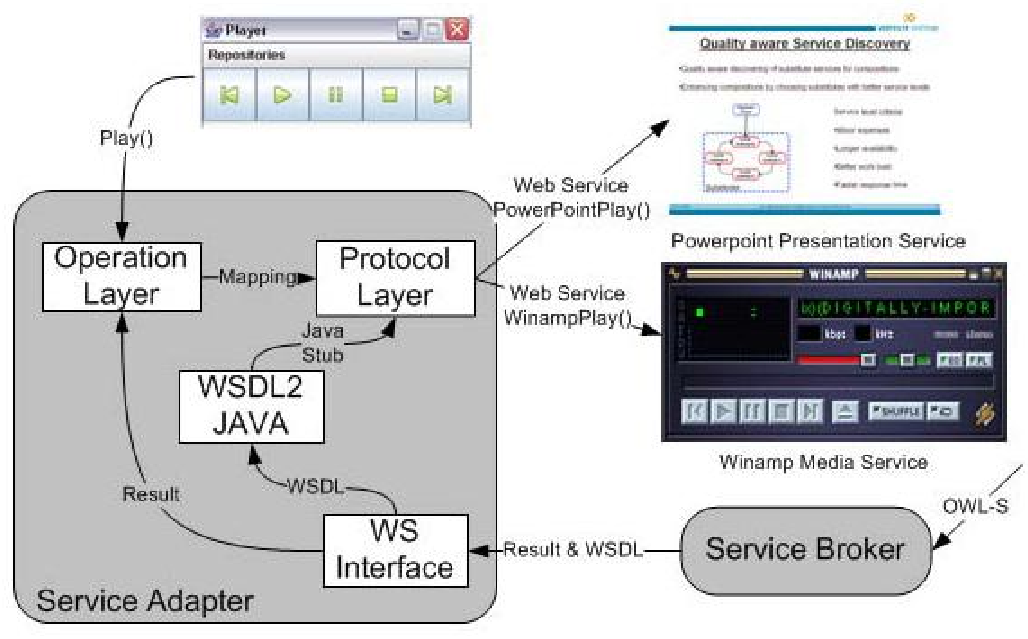
\includegraphics[width=0.85\textwidth]{media/addo-player-example.png}
    \caption{\emph{Referenz-Implementation des \ac{ADDO}-Projektes} \cite[S.418]{flexbrok}.}
    \label{f:addo-player}
}
\end{figure}

Das \ac{ADDO}-Projekt hat zur Verdeutlichung der Zusammenarbeit der vorgestellten Komponenten eine einfache Beispiel-Anwendung implementiert (siehe Abbildung~\ref{f:addo-player} auf Seite~\pageref{f:addo-player}). Die Anwendung ist ein einfaches Multimedia-Player-Frontend, das in Java implementiert ist. Der Player erfordert einen Service, der die Operationen \emph{Play}, \emph{Stop} und \emph{NextTitle} zur Verfügung stellt, sowie optional noch zusätzlich \emph{Pause} oder \emph{PreviousTitle}. Es stehen zwei Systeme zur Verfügung, die diese Operationen anbieten: ein \emph{PowerPoint}-Laptop, der an einen Beamer angeschlossen ist, sowie ein \emph{WinAmp}-Medien-Player, der an einer Stereo-Anlage angeschlossen ist. Beide Systeme sind über einen eigenen Webservice ansprechbar und implementieren mindestens die Operationen \emph{Play}, \emph{Stop} und \emph{NextTitle}. Ihre semantische Beschreibung liegt als \ac{OWL-S} im \emph{Service Broker} vor. Der \emph{Service Container} ist als Java-Bibliothek implementiert und steht in der Anwendung als Instanz zur Verfügung. Ziel ist es nun, einen generischen Medien-Player an die in der aktuellen Umgebung verfügbaren Operationen zu binden. Sobald der \emph{Service Container} von der Anwendung aufgerufen wird, löst die bis jetzt leere Bindung den \emph{Broker}-Mechanismus aus und entweder der \emph{PowerPoint}- oder der \emph{WinAmp}-Webservice wird durch den \emph{Service Broker} gebunden. Der gebundene Dienst wird an den \emph{Service Container} übergeben. Mit Hilfe eines \emph{ant}-Scripts auf Basis von \emph{WSDL2JAVA} wird automatisch ein passender Service-Stub generiert, der die verfügbaren Operationen entsprechend der Webservice-Beschreibung, die in \ac{WSDL} vorliegt, konfiguriert und anschließend in den \emph{Service Container} integriert. Im Fall einer Service-Änderung (Wegfall eines gebundenen Services) wird eine Exception geworfen und die Anwendung kann entweder die Verwendung abbrechen oder einen neuen Service verwenden.

\bigskip

Die hier genannten Beispiel zeigen, dass es bereits funktionsfähige Implementierungen einer Architektur gibt, die in der Lage ist, Services zur Laufzeit zu binden.